\documentclass[aspectratio=169]{beamer}

\usetheme{DUNE}
\beamertemplatenavigationsymbolsempty
\setbeamertemplate{frametitle}{\insertframetitle}

\usepackage[T1]{fontenc}
\usepackage[utf8]{inputenc}
\usepackage{graphicx,booktabs,array,hyperref}
\usepackage{amsmath}
\usepackage{siunitx}
\usepackage{appendixnumberbeamer}
\usepackage[dvipsnames]{xcolor}

\title[daphne-firmware Overview]{Understanding \texttt{daphne-firmware}}
\subtitle{Architecture, build flow, verification strategy, and trigger studies}
\author{Manuel Arroyave}
\date{April 2026}

\begin{document}

\begin{frame}
  \titlepage
\end{frame}

\begin{frame}{What this repo is}
\small
\textbf{One-sentence version}
\begin{itemize}
  \item \texttt{daphne-firmware} is the repository that turns the historical DAPHNE mezzanine Vivado design into something that can be built, reasoned about, verified, and eventually refactored without losing the working hardware path.
\end{itemize}

\vspace{1mm}
\textbf{Why it exists}
\begin{itemize}
  \item The starting point was a working but monolithic firmware tree.
  \item The immediate goal was \textbf{not} a rewrite. The goal was to preserve the shipped path while making the design understandable and testable in pieces.
  \item The repo therefore contains both:
  \begin{itemize}
    \item the imported compatibility lane under \texttt{ip\_repo/} and \texttt{xilinx/}
    \item the newer repo-owned modular, FuseSoC, and formal layers
  \end{itemize}
\end{itemize}
\end{frame}

\begin{frame}{Where we started}
\small
\begin{itemize}
  \item The original firmware lived as a large Vivado-centered codebase with implicit source lists, generated IP dependencies, and subsystem boundaries that were mostly tribal knowledge.
  \item That structure is normal for a lab firmware project, but it makes review, reproducibility, regression isolation, and verification unnecessarily difficult.
  \item The project started from one hard constraint:
  \begin{itemize}
    \item \textbf{do not break the working K26C path while making the design cleaner.}
  \end{itemize}
  \item In practice, this means the migration strategy is additive:
  \begin{itemize}
    \item preserve the qualified implementation flow,
    \item expose explicit boundaries,
    \item add local tests and proofs,
    \item replace internals only after the boundary is explicit.
  \end{itemize}
\end{itemize}
\end{frame}

\begin{frame}{Purpose of the development}
\small
\textbf{Engineering objective}
\begin{itemize}
  \item Convert a monolithic firmware image into a maintainable hardware/software artifact with a stable build contract.
\end{itemize}

\vspace{1mm}
\textbf{Concrete sub-goals}
\begin{itemize}
  \item keep the K26C hardware image buildable and deployable;
  \item make board, feature, and test intent explicit;
  \item isolate analog, frontend, timing, trigger, and transport ownership;
  \item make leaf-level control behavior proof-friendly;
  \item document the build from \texttt{git clone} to \texttt{.bit/.bin/.xsa/.dtbo}.
\end{itemize}

\vspace{1mm}
\textbf{Working rule}
\[
\text{ship path alive} \;\land\; \text{boundary explicit} \;\land\; \text{verification added first}
\]

\vspace{1mm}
This is why the repo has both a compatibility layer and a modular layer.
\end{frame}

\begin{frame}{What we achieved}
\small
\begin{itemize}
  \item Imported the existing firmware tree into a versioned repo with explicit board and platform metadata.
  \item Added FuseSoC cores for platform, feature, smoke-test, and formal targets.
  \item Added repo-owned subsystem wrappers under \texttt{rtl/isolated/}.
  \item Added formal harnesses for control and boundary contracts.
  \item Added repo-owned DT overlay packaging and deployment artifacts.
  \item Documented both a native Linux build path and a WSL + Windows toolchain path.
  \item Validated the operational baseline on hardware:
  \begin{itemize}
    \item routed-clean baseline: \texttt{a389fcd}
    \item current \texttt{main}: \texttt{64d38d1}
    \item overlay load, clock bring-up, \texttt{daphne-server}, oscilloscope mode
  \end{itemize}
  \item This repo is now more than documentation and scaffolding: it owns a real build-to-overlay workflow.
\end{itemize}
\end{frame}

\begin{frame}{Why FuseSoC}
\small
\textbf{Problem}
\begin{itemize}
  \item A pure Vivado project is a poor long-term source-of-truth for a modular firmware project.
\end{itemize}

\vspace{1mm}
\textbf{FuseSoC gives us}
\begin{itemize}
  \item explicit source graphs;
  \item board/platform manifests;
  \item target selection for smoke, formal, and implementation;
  \item less dependence on hand-maintained file lists;
  \item a place to express intent above vendor Tcl.
\end{itemize}

\vspace{1mm}
\textbf{The point is not ideology}
\begin{itemize}
  \item Vivado still performs implementation.
  \item FuseSoC owns the \emph{description of what we mean to build}.
\end{itemize}

\vspace{1mm}
\[
\text{intent layer} \rightarrow \text{source graph} \rightarrow \text{implementation flow}
\]
\end{frame}

\begin{frame}{Why formal verification}
\small
\textbf{What formal is used for here}
\begin{itemize}
  \item not for proving the entire imported design,
  \item but for proving small, stable contracts at boundaries and AXI-lite leaves.
\end{itemize}

\vspace{1mm}
\textbf{Why this matters}
\begin{itemize}
  \item During migration, most bugs are not ``DSP math is wrong'' bugs.
  \item They are reset, gating, readback, enable, and illegal-write bugs.
  \item Those are exactly the cases formal handles well.
\end{itemize}

\vspace{1mm}
\textbf{Examples already covered}
\begin{itemize}
  \item threshold register semantics,
  \item frontend and trigger readiness gates,
  \item analog-control, timing, and Hermes boundary contracts,
  \item delay-line replacement contracts.
\end{itemize}

\vspace{1mm}
\[
\text{assumptions} \Rightarrow \text{guarantees}
\]

\vspace{1mm}
The value is that subsystem behavior becomes explicit before the subsystem is rewritten.
\end{frame}

\begin{frame}{Module map}
\footnotesize
\setlength{\tabcolsep}{5pt}
\begin{tabular}{>{\raggedright\arraybackslash}p{0.28\linewidth} >{\raggedright\arraybackslash}p{0.66\linewidth}}
\toprule
\textbf{Module} & \textbf{Responsibility} \\
\midrule
Control plane & PS-visible register map, AXI-lite leaves, stable software contract \\
Analog/frontend control & AFE and DAC configuration, configuration-ready semantics \\
Frontend boundary & LVDS deserialization, IDELAY/bitslip, trusted alignment promotion \\
Timing subsystem & endpoint timing ingress, clock selection, lock/ready/timestamp validity \\
Trigger pipeline & filters, self-trigger logic, thresholds, peak descriptors, STC3 record build \\
Transport / Hermes & packet export and Ethernet-linked readout transport \\
Verification layer & smoke tests, formal contracts, boundary assertions, build checks \\
\bottomrule
\end{tabular}

\vspace{1mm}
\textbf{Repository organization}
\begin{itemize}
  \item Imported compatibility path: \texttt{ip\_repo/}, \texttt{xilinx/}
  \item Modular repo-owned path: \texttt{rtl/isolated/}, \texttt{cores/}, \texttt{formal/}, \texttt{docs/}
\end{itemize}
\end{frame}

\begin{frame}{Build flow}
\centering
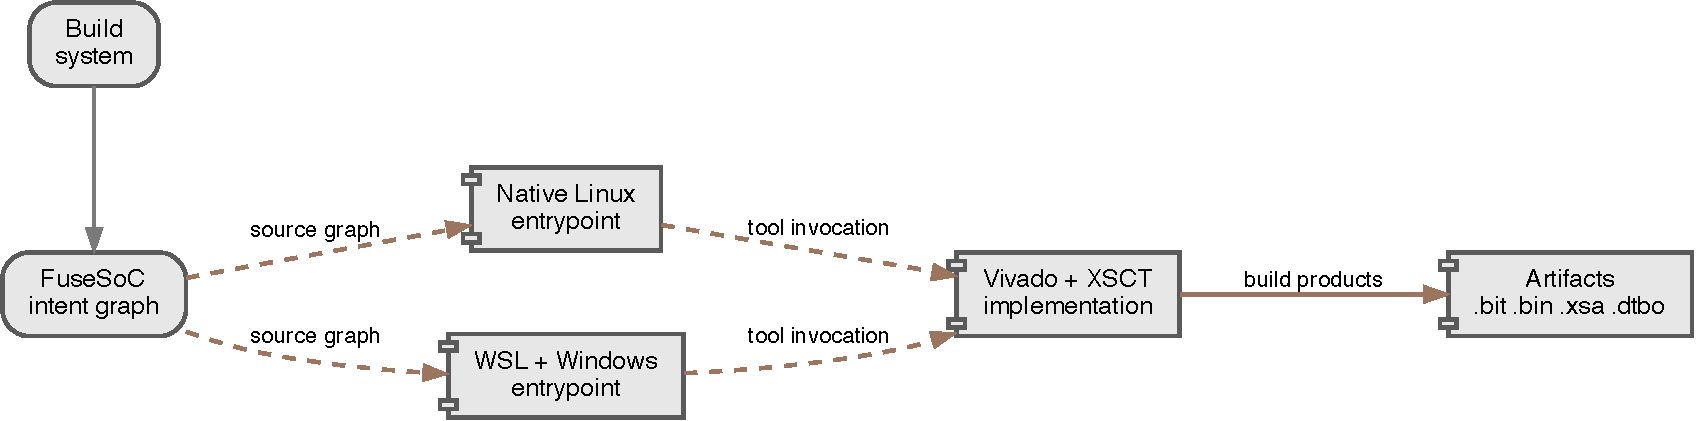
\includegraphics[width=\linewidth,height=0.77\textheight,keepaspectratio]{../daphne_firmware_architecture_assets/output/build_flow_cropped.pdf}
\end{frame}

\begin{frame}{Runtime acquisition path}
\centering
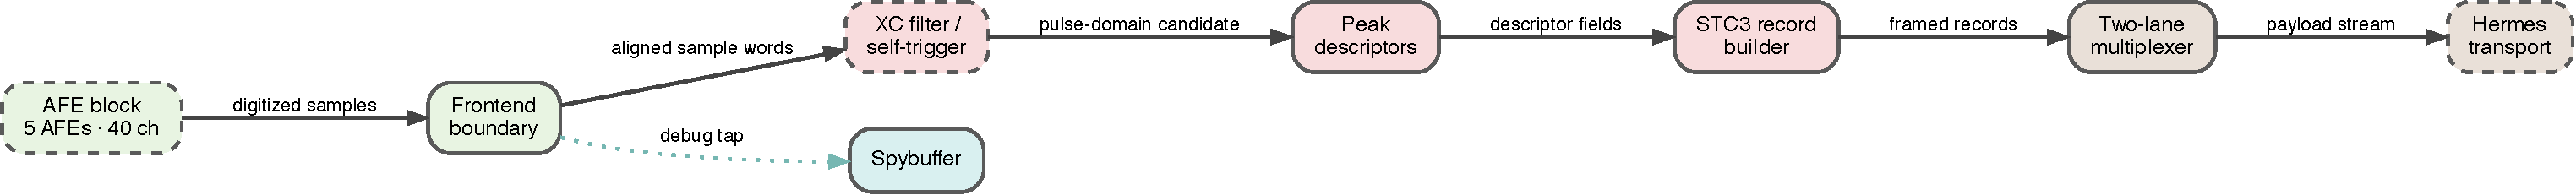
\includegraphics[width=\linewidth,height=0.77\textheight,keepaspectratio]{../daphne_firmware_architecture_assets/output/runtime_dataflow_cropped.pdf}
\end{frame}

\begin{frame}{Clock and timing topology}
\centering
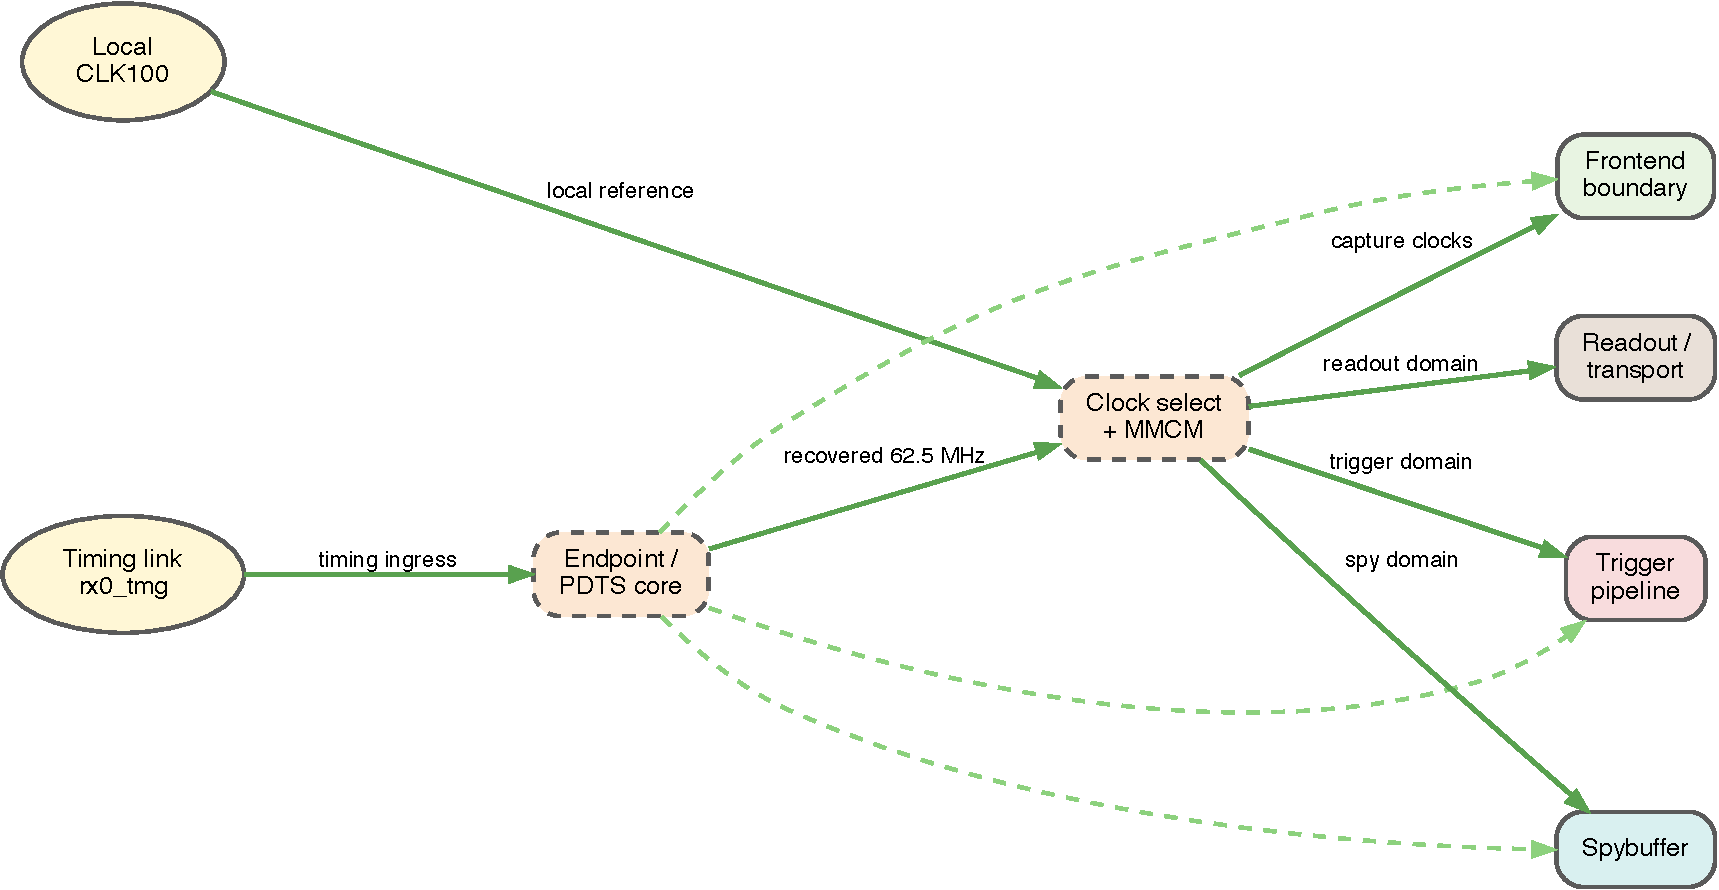
\includegraphics[width=\linewidth,height=0.77\textheight,keepaspectratio]{../daphne_firmware_architecture_assets/output/clock_topology_cropped.pdf}
\end{frame}

\begin{frame}{Readiness contracts}
\centering
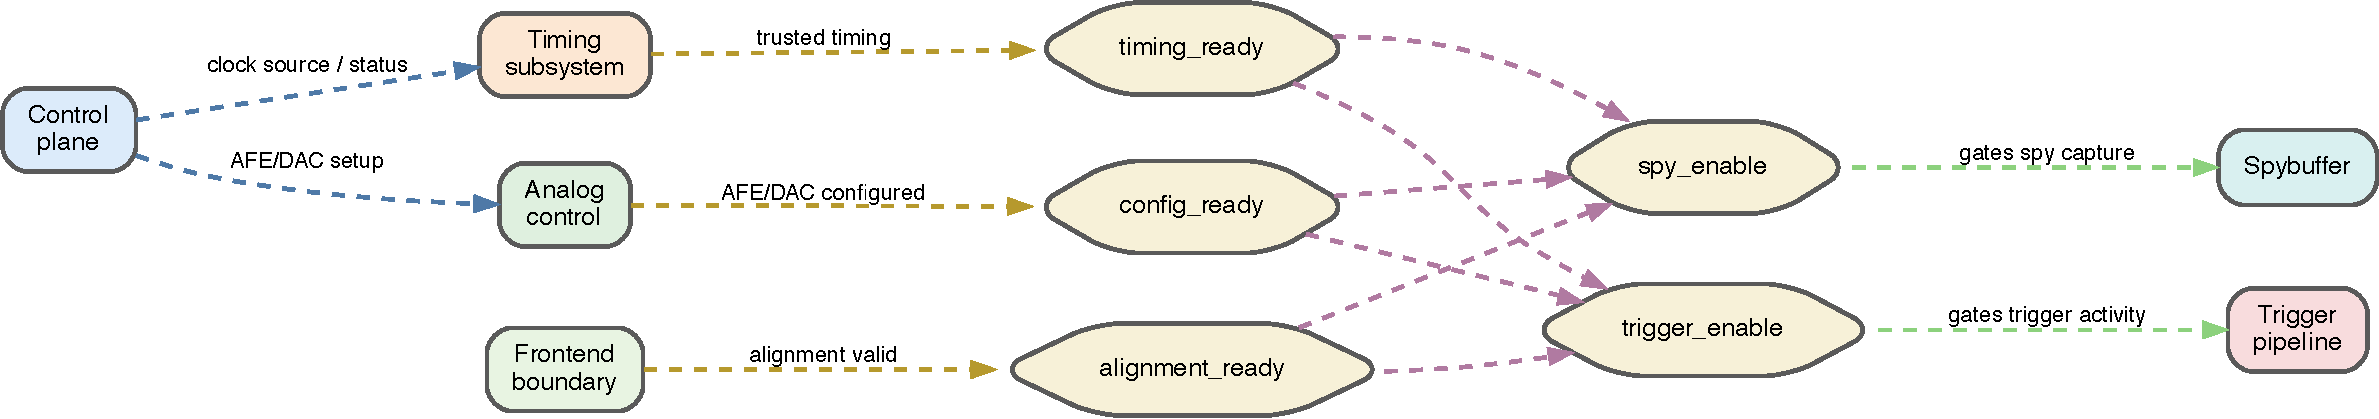
\includegraphics[width=\linewidth,height=0.77\textheight,keepaspectratio]{../daphne_firmware_architecture_assets/output/readiness_contracts_cropped.pdf}
\end{frame}

\begin{frame}[fragile]{Build on a pure Linux machine}
\scriptsize
\textbf{Path rule}
\begin{itemize}
  \item clone to a short path such as \texttt{\~/w/d}
  \item avoid spaces and deep nested directories
\end{itemize}

\vspace{1mm}
\textbf{Clone + build}
\begin{verbatim}
mkdir -p ~/w
git clone git@github.com:DUNE-DAQ/daphne-firmware.git ~/w/d
cd ~/w/d
export XILINX_SETTINGS_SH=/path/to/Vivado/2024.1/settings64.sh
export XILINX_VITIS_SETTINGS_SH=/path/to/Vitis/2024.1/settings64.sh
export DAPHNE_BOARD=k26c DAPHNE_ETH_MODE=create_ip
./scripts/remote/run_remote_vivado_chain.sh
\end{verbatim}

\textbf{Expected output}
\begin{itemize}
  \item \texttt{xilinx/output-<gitsha>/} with \texttt{.bit}, \texttt{.bin}, \texttt{.xsa}, \texttt{.dtbo}, overlay zip, and timing reports
\end{itemize}
\end{frame}

\begin{frame}[fragile]{Build on Windows + WSL}
\scriptsize
\textbf{Qualified arrangement}
\begin{itemize}
  \item shell in WSL2
  \item Vivado 2024.1 and Vitis 2024.1 installed on Windows
  \item short mirrored path: \texttt{C:\textbackslash w\textbackslash d} and \texttt{/mnt/c/w/d}
\end{itemize}

\vspace{1mm}
\textbf{Clone in WSL}
\begin{verbatim}
mkdir -p /mnt/c/w
git clone git@github.com:DUNE-DAQ/daphne-firmware.git /mnt/c/w/d
cd /mnt/c/w/d
export DAPHNE_BOARD=k26c DAPHNE_ETH_MODE=create_ip
./scripts/wsl/check_windows_xilinx.sh
./scripts/wsl/run_wsl_vivado_chain.sh
\end{verbatim}

\textbf{Why the short path matters}
\begin{itemize}
  \item Vivado, DTG, and generated IP trees create very deep paths.
  \item Short paths reduce avoidable tool failures.
\end{itemize}
\end{frame}

\begin{frame}{Mathematical model: baseline and filter preprocessing}
\small
\begin{itemize}
  \item Let \(x[n]\) be the sampled AFE waveform.
  \item The trigger path first estimates a slow baseline and then forms a pulse-domain signal for triggering and descriptors.
\end{itemize}

\vspace{1mm}
\textbf{Firmware low-pass baseline tracker}
\[
b[n] = b[n-1] + 2^{-k}\bigl(x[n] - b[n-1]\bigr), \qquad k = 26
\]

\begin{itemize}
  \item This is the behavior of \texttt{k\_low\_pass\_filter.v}.
  \item It is a very slow IIR baseline estimator.
\end{itemize}

\vspace{1mm}
\textbf{Centered / high-pass view}
\[
d[n] \approx x[n] - b[n]
\]

\begin{itemize}
  \item Depending on configuration, the polarity may be inverted before the matched filter and descriptor stages.
\end{itemize}
\end{frame}

\begin{frame}{Mathematical model: matched filter and self-trigger}
\small
\textbf{Cross-correlation stage}
\[
y[n] = \sum_{i=0}^{31} h[i]\,d[n-i]
\]

\begin{itemize}
  \item \(h[i]\) is the fixed 32-tap template in \texttt{st\_xc.vhd}.
  \item The RTL uses a transposed FIR structure with pipeline registers matching the DSP chain.
\end{itemize}

\vspace{1mm}
\textbf{Trigger condition}
\[
\mathrm{trig}[n] = 1
\]
when \(y[n] > T\), \(y[n-1] > T\), and \(y[n-2] \le T\).

\begin{itemize}
  \item This makes the trigger a one-cycle pulse on a threshold crossing that persists for two consecutive samples.
  \item In the integrated path, this condition is then combined with optional ad-hoc triggers and a fixed latency delay.
\end{itemize}
\end{frame}

\begin{frame}{Mathematical model: peak descriptors}
\small
\textbf{Purpose}
\begin{itemize}
  \item Once a pulse is detected, the descriptor path compresses the waveform into metadata useful for higher-level filtering and transport.
\end{itemize}

\vspace{1mm}
\textbf{Peak-detection logic}
\[
s[n] = x[n] - x[n-L], \qquad L \in \{16,20\}
\]
\[
\text{peak if } s[n] \le \theta_s
\]

\begin{itemize}
  \item This is the slope-threshold logic in \texttt{PeakDetector\_SelfTrigger.vhd}.
  \item An FSM inhibits immediate retriggering until the slope recovers.
\end{itemize}

\vspace{1mm}
\textbf{Descriptor observables}
\[
A_{\max} = \max_t\{-a[t]\}, \quad
t_{\max} = \arg\max_t\{-a[t]\}
\]
\[
Q = \sum_t \max(0,-a[t]), \quad
W = \text{samples in detection window}, \quad
N_{\text{pk}} = \text{count of detected peaks}
\]

\begin{itemize}
  \item Here \(a[t]\) is the signed pulse-domain signal; the current implementation accumulates negative excursions.
  \item The exported metadata are \texttt{ADC\_Peak}, \texttt{ADC\_Integral}, \texttt{Time\_Peak}, \texttt{Time\_Over\_Baseline}, and \texttt{Number\_Peaks}.
\end{itemize}
\end{frame}

\begin{frame}{XC emulation: what it is and what it is not}
\small
\begin{itemize}
  \item The repo \texttt{daphne\_mezz\_xc\_sim} contains a C++ model of the xcorr self-trigger path.
  \item It mirrors:
  \begin{itemize}
    \item the 32-tap transposed FIR,
    \item the trigger condition,
    \item the baseline LPF option,
    \item the CFD gate,
    \item the CIEMAT descriptor path.
  \end{itemize}
  \item This is useful for:
  \begin{itemize}
    \item rapid waveform studies,
    \item threshold and latency scans,
    \item testing trigger logic without full implementation.
  \end{itemize}
  \item It intentionally does \textbf{not} model:
  \begin{itemize}
    \item Ethernet transport,
    \item full shared-lane arbitration.
  \end{itemize}
\end{itemize}
\end{frame}

\begin{frame}{RTL trigger studies: dead time as a system property}
\small
\textbf{Question}
\begin{itemize}
  \item If every channel sees the same nominal offered trigger rate, what dead time per channel should we expect?
\end{itemize}

\vspace{1mm}
\textbf{Two complementary approaches}
\begin{enumerate}
  \item \textbf{Nominal stochastic model}
  \begin{itemize}
    \item uses the measured RTL constants for builder busy time and shared-lane service;
    \item scans the accepted dead fraction versus offered rate.
  \end{itemize}
  \item \textbf{HDL multichannel bench}
  \begin{itemize}
    \item instantiates the real record builder and mux logic;
    \item drives 40 channels with independent arrivals;
    \item measures accepted, dropped, and sent records.
  \end{itemize}
\end{enumerate}

\vspace{1mm}
\textbf{Nature of the test}
\begin{itemize}
  \item This is a \emph{steady-state queueing study} of the trigger and readout chain.
\end{itemize}
\end{frame}

\begin{frame}{Trigger-study result: model versus RTL}
\centering
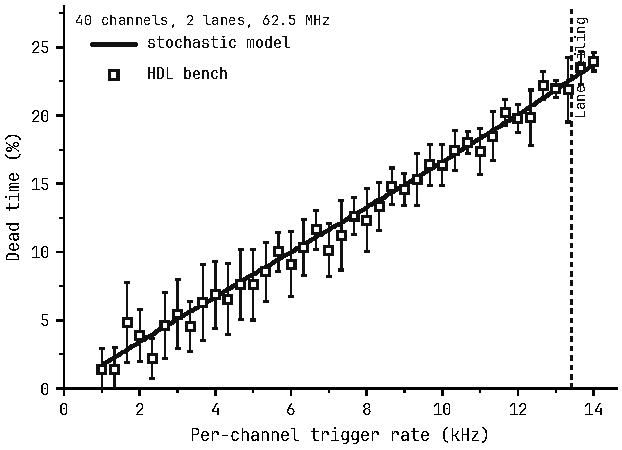
\includegraphics[width=\linewidth,height=0.73\textheight,keepaspectratio]{figures/deadtime_vs_rate_daphne_jetbrains_blackink_40pt_r8.pdf}

\vspace{0.5mm}
\scriptsize
Nominal model against the HDL 40-point, 8-repeat multichannel bench.
HDL markers show the per-rate mean dead fraction, with sample standard deviation across repeats as the error bar.
The same bench summary also stores mean/std for accepted, sent, busy-drop, and full-drop totals at each rate.
\end{frame}

\begin{frame}{Residual view: where the model departs from RTL}
\centering
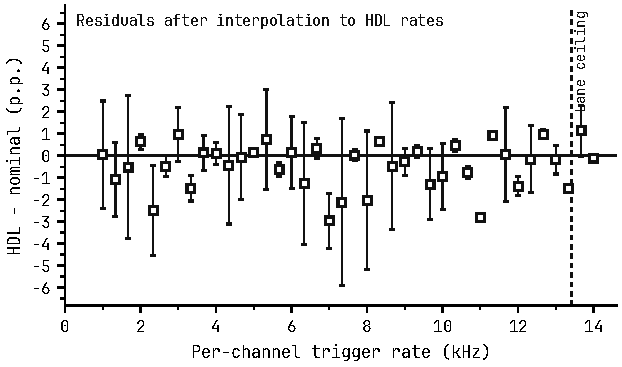
\includegraphics[width=\linewidth,height=0.73\textheight,keepaspectratio]{figures/deadtime_residuals_40pt.pdf}

\vspace{0.5mm}
\scriptsize
Residuals are plotted as \(\Delta(r) = \bar{f}_{\mathrm{HDL}}(r) - f_{\mathrm{nominal}}(r)\) after interpolation of the nominal curve onto the HDL rate points.
The y-error bars reuse the HDL pointwise sample standard deviation; for the current scan,
\(\langle |\Delta| \rangle \approx \num{0.83}\,\text{p.p.}\) and \(\max |\Delta| \approx \num{2.97}\,\text{p.p.}\)
\end{frame}

\begin{frame}{Scope and limits}
\small
\textbf{Operational scope}
\begin{itemize}
  \item qualified board path: K26C
  \item operational routed-clean baseline: \texttt{a389fcd}
  \item current repo tip: \texttt{main} at \texttt{64d38d1}
\end{itemize}

\vspace{1mm}
\textbf{Signal-model assumptions}
\begin{itemize}
  \item baseline subtraction is slow relative to pulse width;
  \item trigger decisions operate on a filtered pulse domain.
\end{itemize}

\vspace{1mm}
\textbf{Dead-time-study assumptions}
\begin{itemize}
  \item homogeneous offered rate across channels;
  \item independent arrivals in the baseline study;
  \item steady-state measurement after warm-up.
\end{itemize}
\end{frame}

\begin{frame}{What to remember}
\small
\begin{itemize}
  \item \texttt{daphne-firmware} is a migration repo with one central rule: preserve the working hardware path while making the design understandable and verifiable.
  \item FuseSoC gives the source and target graph; Vivado still performs implementation.
  \item Formal is used where it is cost-effective: contracts, gates, and AXI-lite/control seams.
  \item The trigger path is algorithmic, not ad hoc:
  \begin{itemize}
    \item slow baseline estimate,
    \item matched-filter trigger,
    \item descriptor extraction,
    \item framed transport through shared readout lanes.
  \end{itemize}
  \item The repo now contains both:
  \begin{itemize}
    \item a hardware-proven build/deploy baseline,
    \item and the analytical + HDL tools needed to study trigger behavior at RTL level.
  \end{itemize}
\end{itemize}
\end{frame}

\end{document}
